\documentclass[border=4pt]{standalone}
% Preámbulo común de las figuras. Cada figura es un documento standalone
% que se compila a SVG con scripts/build_figures.sh
\usepackage[utf8]{inputenc}
\usepackage{amsmath}
\usepackage{tikz}
\usepackage[american, siunitx]{circuitikz}
\usetikzlibrary{arrows.meta,calc,decorations.pathmorphing,patterns}
\tikzset{
  >={Stealth[length=2.2mm]},
  eje/.style={->, thin},
  hilo/.style={thick},
}
% Paleta común: tonos medios legibles sobre fondo claro
\definecolor{azul}{RGB}{31,94,168}
\definecolor{rojo}{RGB}{192,57,43}
\definecolor{verde}{RGB}{39,128,73}
\definecolor{naranja}{RGB}{211,120,30}
\definecolor{morado}{RGB}{125,60,152}

\begin{document}
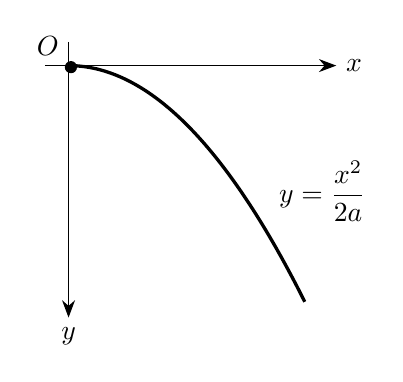
\begin{tikzpicture}[scale=1.0]
  \draw[eje] (-0.3,0) -- (3.4,0) node[right]{$x$};
  \draw[eje] (0,0.3) -- (0,-3.2) node[below]{$y$};
  \node[above left] at (0,0) {$O$};
  \draw[very thick] plot[domain=0:3.0, samples=60] (\x, {-\x*\x/3});
  \fill (0.03,-0.02) circle (2.2pt);
  \node[right] at (2.55,-1.6) {$y = \dfrac{x^2}{2a}$};
\end{tikzpicture}
\end{document}
